\vspace{-10pt}
\section{Preliminaries}
\label{sec:preliminaries}
\vspace{-7pt}

\noindent\textbf{Self-Supervised Learning.}
The training procedure of several state-of-the-art SSL methods \cite{zbontar2021barlow,chen2020simple,he2020momentum,caron2020unsupervised,caron2021emerging,bardes2021vicreg, dwibedi2021little,grill2020bootstrap} can be summarized as follows. Given an image $\xvect$ in a batch sampled from a distribution $\mathcal{D}$, two correlated views $\xvect^A$ and~$\xvect^B$ are extracted by applying stochastic image augmentations, such as random cropping, color jittering and horizontal flipping. View $\xvect^A$ is fed to an encoder $f_\theta = f_p \circ f_b$, which is parametrized by $\theta$ and has a backbone $f_b$ and a projection head $f_p$, that  extracts feature representations $\zvect^A = f_\theta(\xvect^A)$. Similarly, $\xvect^B$ is forwarded into the same networks, or possibly copies thereof, updated with exponential moving average (EMA), to obtain the representation~$\zvect^B$. A loss function $\mathcal{L}_{SSL}$ is applied to these representations to learn the parameters $\theta$ as follows:
\begin{equation}
\label{eq:ssl_obj}
    \underset{\theta}{\operatorname{argmin}} \,\, \mathbb{E}_{\xvect \sim \mathcal{D}}\left[\mathcal{L}_{SSL}\left(\zvect^A, \zvect^B\right)\right].
\end{equation}
More details on the implementation of $\mathcal{L}_{SSL}$ are provided in Sec.~\ref{sec:compatibility} and Tab.~\ref{tab:methods}. This procedure turns out to be extremely powerful at extracting visual representations from large unlabeled datasets. The intuition behind the success of these models is that they learn to be invariant to augmentations. Importantly, augmentations are hand-crafted in a way that the two views $\xvect^A$ and $\xvect^B$ contain roughly the same semantics as $\xvect$, but their overall appearance (geometry, colors, resolution, \etc) is different. This forces the model map images with the same semantics to similar regions of the feature space. Interestingly, these augmentations are much stronger, \ie, they distort the image more, than augmentations commonly used to train supervised models.

\noindent\textbf{Continual Learning.}
The CL problem focuses on training models such as deep neural networks from non-stationary data distributions. More formally, this involves a network $f^{\prime}_{\theta^{\prime}} = f^{\prime}_c \circ f^{\prime}_b $ with parameters $\theta^{\prime}$, backbone $f^{\prime}_b$ and a classifier $f^{\prime}_c$, that learns from an ordered set of tasks $\{1,\dots, T\}$, each exhibiting a different data distribution $\mathcal{D}_t$. Usually, an image $\xvect$ sampled i.i.d.\ from $\mathcal{D}_t$ is processed by $f^{\prime}$ that predicts a probability distribution $\pvect$ over the set of classes $\mathcal{Y}_t$. The objective is to find parameters $\theta^{\prime}$ such as:
\begin{equation}
\label{eq:cl_obj}
\underset{\theta^{\prime}}{\operatorname{argmin}} \sum_{t=1}^{T} \mathbb{E}_{(\xvect, \yvect) \sim \mathcal{D}_{t}}\left[\mathcal{L}_{CL}\left(\pvect, \yvect\right)\right],
\end{equation}
where, in most cases, $\mathcal{L}_{CL}$ is the cross-entropy loss. However, during task $t$, the previous data distribution $\mathcal{D}_{t-1}$ is not available and therefore Eq.~(\ref{eq:cl_obj}) cannot be minimized directly. Current research focuses on approximating $\theta^{\prime}$ using indirect approaches. Some of them~\cite{Li17learning, douillard2020podnet} are based on knowledge distillation~\cite{hinton2015distilling}, \ie, transferring knowledge from one network to another by forcing them to produce the same outputs. We will discuss the applicability of distillation methods in CSSL in Sec.~\ref{sec:cassowary}.

\vspace{-5pt}
\section{Continual Self-Supervised Learning}
\label{sec:cssl}
In this paper, we tackle the problem of Continual Self-Supervised Learning 
as an extension of both SSL and CL.
In practice, a CSSL experiment starts with the first task, where the model is trained as per the specific self-supervised method that it implements, with no difference from offline training. Subsequent tasks are then presented to the model sequentially, and the data from the previous tasks are discarded.
No labels are provided during this training phase. For the sake of simplicity and since we are exploring a new, challenging setting, we assume task boundaries to be provided to the model.
More formally, the CSSL objective is to learn a strong feature extractor that is invariant to augmentations on all tasks. Following the notation introduced in Sec.~\ref{sec:preliminaries},  we define: 
\begin{equation}
\label{eq:continual_erm}
\underset{\theta}{\operatorname{argmin}} \sum_{t=1}^{T} \mathbb{E}_{\xvect \sim \mathcal{D}_{t}}\left[\mathcal{L}_{SSL}\left(\zvect^A, \zvect^B\right)\right].
\end{equation}
Note the absence of labels $\yvect$ when sampling from $\mathcal{D}_t$, the summation over the set of tasks inherited from Eq.~(\ref{eq:cl_obj}) and the SSL loss function in Eq.~(\ref{eq:ssl_obj}). The expectation is approximated using stochastic gradient descent on minibatches.

\noindent\textbf{Evaluation.} After each task, it is possible (for evaluation purposes) to train a linear classifier on top of the obtained backbone $f_b$. With this linear classifier we report accuracy on the test set. This protocol is compatible with standard CL metrics, as shown in Sec.~\ref{sec:protocol}.
We explore three CSSL settings in our work.\\
\mybullet\ \textbf{Class-incremental}: each task $t$ is represented by a dataset $D_t \sim \mathcal{D}_t$ containing images that belong to a set of classes $\mathcal{Y}_t$ such that $\mathcal{Y}_t \cap \mathcal{Y}_s = \varnothing$ for each other task $s \neq t$. Note that the class labels are only used for splitting the dataset and they are unknown to the model. In practice, the set of classes in the dataset are shuffled and then partitioned into $T$ tasks. Each task contains the same number of classes.\\
\mybullet\ \textbf{Data-incremental}: each task $t$ contains a set of images $D_t$ such that $D_t \cap D_s = \varnothing$ for each other task $s \neq t$. No additional constraints are imposed on the classes. In practice, the whole dataset is shuffled and then partitioned into $T$ tasks. Each task can potentially contain all the classes. \\
\mybullet\ \textbf{Domain-incremental}: each task $t$ contains a set of images $D_t$ drawn from a different domain. We assume that the set of classes $\mathcal{Y}_t$ in each dataset remains the same for all tasks but the data distribution changes, as if the data were collected from different sources. 
\vspace{-5pt}
\section{The \name{} Framework}
\label{sec:cassowary}
\vspace{-5pt}
We now introduce ``\name{}'', our framework for 
continual self-supervised learning of visual representations and detail its compatibility with several SSL methods.
\vspace{2pt}

\noindent{\bf Distillation in CSSL.} From a supervised CL perspective, the concept of invariance is interesting. Here, we would like to learn representations of previously-learned semantic concepts that are invariant to the state of the model's parameters. 
Indeed, this idea was investigated in prior works~\cite{douillard2020podnet, hou2019learning} that leverage knowledge distillation for CL. However, such approaches are only  mildly effective in a CSSL scenario, as we show in Sec.~\ref{sec:experiments}. 
We believe this is due to CSSL being fundamentally different from supervised CL. In CSSL, we aim to extract the best possible representations that can be subsequently reused in a variety of tasks, and maximize the linear separability of features at the end of the CL phase. Thus, the linear classifier does not benefit much from the stability of the representations. Also, forcing the representations not to change may prevent the model from learning new concepts. 
This is especially critical for SSL methods for two reasons: (i) the performance of the models improve substantially with longer training, implying that the representations continue to get refined, and (ii) they exhibit different losses and feature normalizations that might interfere with distillation and vice-versa (\eg, BarlowTwins uses standardization while~\cite{douillard2020podnet, hou2019learning} use $l2$-normalization). Nonetheless, the features still need to be informative of previous tasks to maximize the separability of the old distribution but the current state might be too different from the previous one making comparing representations complicated.

\vspace{2pt}
\noindent{\bf Distillation through SSL losses.}
Our framework, shown in Fig.~\ref{fig:\name{}}, is based on the following ideas: (i)~a predictor network that maps the current state of the representations to their past state, by leveraging a distillation through time strategy that satisfies both stability and plasticity principles, and (ii)~a family of adaptable distillation losses inherited from the SSL literature that solves the issue of having different objectives interfering with each other.

\begin{figure}[t]
\centering
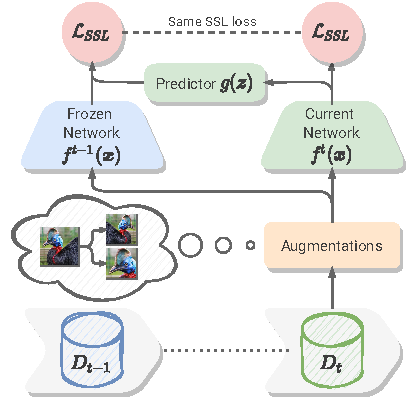
\includegraphics[width=0.85\columnwidth]{figures/name_of_method.pdf}
\vspace{-8pt}
\caption{Overview of the \name{} framework.}
\label{fig:\name{}}
\vspace{-11pt}
\end{figure}

When a new task is received, we start by making a copy of the current model. This copy does not require gradient computation and will not be updated. We call this the \textit{frozen encoder} $f^{t-1}$. As soon as an image $\xvect \in D_t$ is available we apply our stochastic image augmentations and extract its features $\zvect = f^t(\xvect)$. In addition, we also use the frozen encoder to extract another feature vector $\bar{\zvect} = f^{t-1}(\xvect)$. Now, our goal is to ensure that $\zvect$ contains at least as much information as (and ideally more than) $\bar{\zvect}$. Instead of enforcing the two feature vectors to be similar, and hence discouraging the new model from learning new concepts, we propose 
to use a predictor network $g$ to project the representations from the new feature space to the old one. If the predictor is able to perfectly map from one space to the other, then it implies that $\zvect$ is at least as powerful as $\bar{\zvect}$.

We are now ready to perform distillation, but which is the most appropriate distillation loss? 
Since we want the representations produced by $g$ to be invariant to the state of the model, we propose to use the same SSL loss used to simulate invariance to augmentations. Empirically, we verify that this choice reduces interference and minimizes the need for hyperparameter tuning. We can hence write a generic distillation loss by reusing the definition of $\mathcal{L}_{SSL}$:
\begin{equation}
    \mathcal{L}_D(\zvect, \bar{\zvect}) = \mathcal{L}_{SSL} (g(\zvect), \bar{\zvect}).
\end{equation}
Note that $\bar{\zvect}$ is always detached from the computational graph, such that the frozen encoder does not receive any gradient, and the gradient only flows through the predictor $g$, as prescribed in~\cite{chen2021exploring}. On the one hand, if training  converges and $\mathcal{L}_D$ is minimized, the features predicted by $g$ will likely be quasi-invariant to the state of the model, which satisfies the stability principle. On the other hand, the current encoder is less bound to its previous state, hence representations $\zvect$ can be more plastic. The loss can be extended to multiple views by applying it to both representations, \textit{i.e.}, $\mathcal{L}_D(\zvect^A, \bar{\zvect}^A) + \mathcal{L}_D(\zvect^B, \bar{\zvect}^B)$, and also swapped distillation, \textit{e.g.}, $\mathcal{L}_D(\zvect^A, \bar{\zvect}^B)$ and vice-versa (see ablation in Tab.~\ref{tab:ablation}).

The final loss of an SSL method trained continually with the \name{} framework is given by:
\begin{equation}
\begin{aligned}
    \mathcal{L} &= \mathcal{L}_{SSL}(\zvect^A, \zvect^B) + \mathcal{L}_{D}(\zvect^A, \bar{\zvect}^A) \\
    &= \mathcal{L}_{SSL}(\zvect^A, \zvect^B)  +\mathcal{L}_{SSL} (g(\zvect^A), \bar{\zvect}^A).
\end{aligned}
\label{eq:\name{}}
\end{equation}
This loss can be made symmetric by applying it to both the views (swapping $A$ and $B$ in Eq.~(\ref{eq:\name{}})) and it can also be easily adapted for multi-crop~\cite{caron2020unsupervised}. Note that we do not use any hyperparameter to weight the importance of the distillation loss with respect to the SSL loss.


\vspace{-5pt}
\subsection{Compatibility of SSL methods with \name{}}
\label{sec:compatibility}
\vspace{-5pt}
The main difference among SSL methods is the loss function that they use. Following the notation defined in Sec.~\ref{sec:preliminaries}, and the loss functions in Tab.~\ref{tab:methods}, we now detail if and how SSL losses can be used in our \name{} framework. Full derivation of distillation losses is deferred to the supplementary material.

\noindent\textbf{InfoNCE-based} methods \cite{chen2020simple, he2020momentum} perform instance discrimination, where positive samples help to build invariance to augmentations. The negatives prevent the model from falling into degenerate solutions. The InfoNCE (\textit{a.k.a.} contrastive) loss can be written as in Eq.~(\ref{eq:infonce}), where subscript~$i$ is the index of a generic sample in the batch, $\operatorname{sim}$ is the cosine similarity and $\eta(i)$ is the set of negatives for sample $i$ in the current batch. 
Distilling knowledge with this loss is equivalent to performing instance discrimination of current task samples but in the feature space learnt in the past. Thus, the predictor $g$ learns to project samples from the present to the past space to maximize the distance with the negative samples, and the similarity with itself in the past.

\noindent\textbf{MSE-based} approaches~\cite{grill2020bootstrap, chen2021exploring} enforce consistency among positive samples and ignore the negatives. BYOL~\cite{grill2020bootstrap} uses a momentum encoder and SimSiam~\cite{chen2021exploring} performs a stop gradient operation to avoid degenerate solutions. Since the representations are $l2$-normalized, their loss (Eq.~\ref{eq:mse}) can be rewritten as the negative cosine similarity:  $-\operatorname{sim}(\qvect^A, \zvect^B) =-\frac{\qvect^A}{||\qvect^A||_2}\cdot\frac{\zvect^B}{||\zvect^B||_2}$,
where $\qvect^A = h(\zvect^A)$ and $h$ is a prediction head. The gradient is backpropagated only through the representations of the first argumentation. A special case of this family of methods is VICReg~\cite{bardes2021vicreg}, which uses a combination of multiple losses, where MSE acts as invariance term. Features are not $l2$-normalized in VICReg and its predictor is the identity function. In our framework, this loss encourages the model to predict the past state of representations without additional regularization.

\begin{table}[t]
\caption{Overview of state-of-the-art SSL methods and losses. In all tables, highlight colors are coded according to the type of loss.}
\label{tab:methods}
\vspace{-8pt}
\centering
\resizebox{0.99\columnwidth}{!}{
\captionsetup{type=table}
\begin{tabular}{m{1.9cm}ccc}
\toprule
\textbf{Methods} & \textbf{Loss} & \textbf{Equation} \\ 
\midrule
SimCLR~\cite{chen2020simple} & \CC{contrcolor} & \multirow{3}{*}{$-\log \frac{\exp \left(\operatorname{sim}\left(\zvect_i^A, \zvect_i^B\right) / \tau\right)}{\sum_{\zvect_j \in \eta(i)} \exp \left(\operatorname{sim}\left(\zvect_i^A, \zvect_{j}\right) / \tau\right)}$} & \hspace{-3mm} \multirow{3}{*}{$\refstepcounter{equation}(\theequation)\label{eq:infonce}$} \\
MoCo~\cite{he2020momentum} & \CC{contrcolor} \\
NNCLR~\cite{dwibedi2021little} & \CC{contrcolor} \multirow{-3}{*}{InfoNCE} \\\midrule

BYOL~\cite{grill2020bootstrap} &  \CC{predcolor} & \multirow{3}{*}{$-||\qvect^A -  \zvect^B||^2_2$} & \hspace{-3mm}\multirow{3}{*}{$\refstepcounter{equation}(\theequation)\label{eq:mse}$} \\
SimSiam~\cite{chen2021exploring} & \CC{predcolor}\\
VICReg~\cite{bardes2021vicreg} & \CC{predcolor}\multirow{-3}{*}{MSE}\\\midrule


SwAV~\cite{caron2020unsupervised} & \CC{knowcolor}  & \multirow{3}{*}{$-\sum_{d} \avect_{d}^B \log \frac{\exp \left(\operatorname{sim}\left( \zvect^A, \cvect_{d}\right) / \tau\right)}{\sum_k \exp \left(\operatorname{sim}\left(\zvect^A, \cvect_k\right) / \tau\right)} $} & \hspace{-3mm} \multirow{3}{*}{$\refstepcounter{equation}(\theequation)\label{eq:cross-entropy}$} \\
DCV2~\cite{caron2020unsupervised} & \CC{knowcolor}\\
DINO~\cite{caron2021emerging} & \CC{knowcolor}\multirow{-3}{*}{Cross-entropy} \\\midrule

Barlow Twins~\cite{zbontar2021barlow} &\CC{decorrcolor}  & \multirow{2}{*}{$\sum_{u}\left(1-\mathcal{C}_{u v}\right)^{2}+\lambda \sum_{u} \sum_{v \neq u} \mathcal{C}_{u v}^{2}$} & \hspace{-3mm} \multirow{2}{*}{$\refstepcounter{equation}(\theequation)\label{eq:cross-correlation}$}\\
VICReg~\cite{bardes2021vicreg} &\CC{decorrcolor}\multirow{-3}{*}{Cross-correlation} \\

\bottomrule
\end{tabular}
}
\vspace{-13pt}
\end{table}
\noindent\textbf{Cross-entropy-based.} Instead of simply enforcing invariance of the representations to augmentations, cluster prototypes $\mathbf{C} = \left\{\mathbf{c}_{1}, \ldots, \mathbf{c}_{K}\right\}$ are used as a proxy in these approaches, so that the model learns to predict invariant cluster assignments. Slight variations of this idea result in different methods: SwAV~\cite{caron2020unsupervised}, DeepClusterV2~\cite{caron2020unsupervised} and DINO~\cite{caron2021emerging}. Once a probability distribution over the prototypes is predicted, the cross-entropy loss (Eq.~\ref{eq:cross-entropy}) is used to compare the two views.
Features and cluster prototypes $\cvect$ are $l2$-normalized. The assignments $\avect^B$ can be calculated in several ways, \textit{e.g.}, k-means in DeepCluster, Sinkhorn-Knopp in SwAV and EMA in DINO. When employed as a distillation loss, cross-entropy encourages $g$ to predict the assignments generated by the frozen encoder with a set of frozen prototypes: $\avect^B = \frac{\exp \left(\operatorname{sim}\left( \bar{\zvect}^B, \cvect^{t-1}_{d}\right) / \tau\right)}{\sum_k \exp \left(\operatorname{sim}\left(\bar{\zvect}^B, \cvect^{t-1}_k\right) / \tau\right)}$, where $\mathbf{C}^{t-1} = \left\{\mathbf{c}^{t-1}_{1}, \ldots, \mathbf{c}^{t-1}_{K}\right\}$.

\noindent\textbf{Cross-correlation-based}. These methods use a different approach based on decorrelating the components of the feature space, \textit{e.g.}, Barlow Twins~\cite{zbontar2021barlow}, VICReg~\cite{bardes2021vicreg} and W-MSE~\cite{ermolov2021whitening}. For our analysis, we will mainly focus on Barlow Twins' implementation of this objective. Extensions to VICReg are left for future work. The cross-correlation based objective function is shown in Eq.~\ref{eq:cross-correlation}, 
where $\lambda$ is an hyperparameter to control the importance of the first and the second terms of the loss, and $\mathcal{C}_{u v} = \frac{\sum_{i} \zvect_{i, u}^{A} \zvect_{i, v}^{B}}{\sqrt{\sum_{i}\left(\zvect_{i, u}^{A}\right)^{2}}. \sqrt{\sum_{i}\left(\zvect_{i, v}^{B}\right)^{2}}}$ is the value of position $(u,v)$ of the cross-correlation matrix computed between the representations of the views along the batch dimension. Note that the representations here are mean centered along the batch dimension, such that each unit has mean output zero over the batch. Performing distillation with this loss has the additional effect of decorrelating the dimensions of the predicted features $g(\zvect^A)$.